\documentclass[oneside,a4paper,titlepage]{article}
\usepackage{blindtext}
\usepackage[utf8]{inputenc}
\usepackage{verbatim} 
\usepackage{graphicx}
\usepackage{color}
\usepackage{float}
\usepackage[hidelinks]{hyperref}
\usepackage{lipsum}
\usepackage{pdfpages}

% Mappe hvori billeder ligger
\graphicspath{ {graphics/} }

% Tekst som står først i figur captions "{Figure/Figur} 3: Pixelering der fremkommer..."
\renewcommand{\figurename}{Figur}
\renewcommand{\abstractname}{Abstrakt}
\renewcommand\refname{}


% supresses errors during compilation
% \batchmode

%\title{Ray Tracing}
%\author{P1 B2-28}
%\date{\today}

\begin{document}
%\maketitle

% \begin{abstract}
% Abstract text placeholder, lorem ipsum dolor sit amet...
\clearpage
% \end{abstract}


% sections
\begin{titlepage}
  %\toprule[2pt]
  %\midrule
  \vspace{0.2cm}
  \begin{center}
    \Huge{\textbf{Visualisering af lampers belysning}}
  \end{center}
  \vspace{0.2cm}
  %\midrule
  %\toprule{2pt}
  \vfill
  \begin{center}
  \includegraphics[height=9cm]{front.png}
  \end{center}
  \begin{center}
    \Large{\textbf{Gruppe B2-28}}\\
	Morten Rask Andersen\\
	Anton Christensen\\
	Lasse Fribo Gadegaard\\
	Christian Mønsted Grünberg\\
	Mathias Ibsen\\
	Mathias Rohde Pihl
  \end{center}
  \begin{center}
 	18/12-2015
    Aalborg Universitet\\
    Software, 1. semester
  \end{center}
\end{titlepage}


%Synopsis
\includepdf[page={-},offset=0mm 0mm]{synopsis_p1}
\addtocounter{page}{-1}
\clearpage

\thispagestyle{empty}
\noindent\begin{tabular}{ll}
\makebox[2.5in]{\hrulefill} & \makebox[2.5in]{\hrulefill}\\
Morten Rask Andersen & Anton Christensen\\[8ex]
\makebox[2.5in]{\hrulefill} & \makebox[2.5in]{\hrulefill}\\
Lasse Fribo Gadegaard & Christian Grünberg\\[8ex]
\makebox[2.5in]{\hrulefill} & \makebox[2.5in]{\hrulefill}\\
Mathias Ibsen & Mathias Pihl\\[8ex]
\end{tabular}

\clearpage


\section{Forord}
Denne rapport er udarbejdet af gruppe B2-28, bestående af software-studerende, som P1-rapport på Aalborg Universitet.

Rapporten tager udgangspunkt i Aalborg-modellen for problembaseret læring. Denne læringsproces har givet gruppen mulighed for at undersøge en given problemstilling og derudfra tilegne sig viden, og på baggrund af denne viden udarbejde en problemanalyse. Derudover gør rapporten brug af den kvalitative metode til korrespondance med interessenterne. Den kvalitative metode er fordelagtig at bruge, når man vil undersøge forhold, som er svære at iagttage eller måle \cite{kvalitativ_metode}. I forbindelse med problemanalysen har vi haft kontakt med to lampedesignere og en belysningskonsulent for en dansk lampebutik. Belysningskonsulenten vil efter eget ønske fremgå anonymt. 

Tak til vejledere Benjamin Bjerre Krogh og Annette Grunwald samt den medvirkende belysningskonsulent og de medvirkende designere.

Rapporten er blevet afleveret på papirform og online på Digital Eksamen, hvor programmet er blevet vedhæftet. Koden kan derfor findes online og betragtes som elektronisk bilag. Farvede billeder kan derfor også ses på online udgaven af rapporten. 

Som en del af projektet er der i rapportens appendiks udarbejdet et projektforslag til næste års P1-forløb.
\clearpage
\subsection{Læsevejledning}

Hvert afsnit X.X har sin egen indledning og opsummering hhv.\ først og sidst i afsnittet. Kilder og kodeuddrag er angivet i rapporten, som beskrevet i nedenstående afsnit.

\subsubsection{Kildehenvisning}
Rapportens brug af kildehenvisninger er baseret på nummermetoden. I nummermetoden anføres kilderne i fortløbende nummerorden, svarende til hvilket nummer, de har i teksten. To identiske kilder har samme nummer. Herunder ses et eksempel på hhv. en internetkildehenvisning og en artikel- eller bogkildehenvisning:

Interneteksempel med kilde[1].

[1] Titel på emne eller kort forklaring på emnet, hjemmesidenavn. Set DD-MM-YYYY. URL på hjemmeside.


Bogeksempel med kilde[2].

[2] Titel på bog, forfatter(e), udgivelsesår, udgavenummer. ISBN/ISSN-nummer.


Hvis en kilde har yderligere relevante informationer (såsom sidetal, copyright mm. angives disse også i kilden.


Figurhenvisning foregår på samme måde som med andre kilder, dog med en forklaring under selve figuren. Hvis en figur ingen kilde har, er figuren fremstillet af gruppen.


\subsubsection{Kodeuddrag}
Flere steder i rapporten, vil der blive vist dele af gruppens kode. Et eksempel på hvordan dette vil blive vist er herunder:

\begin{lstlisting}[style=Cstyle, caption=Kodeeksempel i C]
#include <stdio.h>

int main(void){
   printf("Hello, world!\n");
   return 0;
}
\end{lstlisting}

\clearpage

\tableofcontents
\clearpage

\subsection{indledning}

Selvom vi ikke så ofte tænker på det, så er lamper en stor del af vores hverdag. De står i vores hjem, på vores gader, på vores arbejdsplads - ja de er stort set overalt. Men hvorfor er lamper endelig så vigtige? Det er de, fordi lamper bliver brugt til at skabe lys. Belysning kan bidrage til mange ting som at læse og arbejde bedre, eller til at skabe hygge og stemning i et rum der ellers ville have været koldt og kedeligt. Lamper findes i mange forskellige typer og mange forskellige steder. Der er læselamper, arbejdslamper, loftlamper, udendørslamper osv. og de tjener allesammen et forskelligt formål, men fælles for dem er, at de skaber lys steder hvor der ellers ikke ville have været lys. 
I dag findes der utroligt mange forskellige lampedesigns, og de er ikke allesammen lige gode. Heraf menes der at nogle lamper har meget dårlig belysning. Dette er et problem, da undersøgelser har vist at dårlig belysning kan føre til blandt andet øjenskader, hovedpine og falden. Nogle af disse konsekvenser kan også opstå hvis en lampe har en for kraftig belysning, og derfor er blændende eller hvis f.eks en udendørs lampe ikke lyser tilstrækkeligt, og man vælter fordi man ikke kan se noget. 
Så selvom lamper spiller en stor rolle i vores hverdag, så er det vigtigt at kunne visualisere hvordan lys udbreder sig fra en lampe, så man kan undgå dårlig belysning. 
Fordi at lamper i sig selv er et stort emne, der dækker over ting som design, indretning, belysning etc. så har vi valgt at den videre rapport skal beskæftige sig med visualisering af lys fra lamper. 




\section{Problemanalyse}
For at besvare det initierende problem, er det nødvendigt at researche, heraf opstilles der en række HV-spørgsmål, som vil danne grundlag for problemfeltet. Formålet med disse spørgsmål er, at komme i dybden med samt at forstå problemet.  
\newline For at få afklaret hvor stort et problem det egentlig er, vil der blive uddelt spørgeskemaer, med formål at få en idé om omfanget af problemet. 
Spørgeskemaet vil være et redskab, som vi benytter for at få bekræftet vores antagelse om hvorvidt det er svært at visualisere lysets udbredelse fra en lampe. 

\subsection{Relevans}
Rapporten vil i dette afsnit bestræbe sig efter at besvare om problemet er relevant og i så fald, hvorfor det er relevant. I denne sammenhæng ligges der blandt andet fokus på hvordan lyset påvirker mennesker, samt hvilke konsekvenser dårlig belysning kan medføre. 

\subsubsection{Lysets påvirkning på mennesket}

Undersøgelser har vist at lys har stor invirkning på vores humør og trivsel.
Blåt/hvidt lys har den effekt at vi føler os mere vågne og oppe på mærkerne\cite{videnskab_dk_paavirkning}, hvorimod rødt/gult lys har den modsatte effekt. Vi bliver mere afslappede og dermed trætte. Det giver god mening når vi ser på det lys solen udsender om dagen(hvidt/blå himmel), som gør os friske, og det lys vi ser når solen går ned(rød solnedgang/bål om natten) og det er tid til at gå til ro. 
\newline Vi bruger også lys til rigtig meget i hverdagen. Øjet, som virker ved hjælp af lys bruger vi til at navigere, se evt. farer og genkende venner. Når vi bruger en computer er vi afhængige af at kunne se skærmen for at kunne bruge den. 
\newline Mange mennesker sidder i kontormiljøer i stort set al deres arbejdstid og er afhængige af at lyset er godt, jf. indledning. Hvis lyset ikke er godt vil man ofte blive træt og uproduktiv. Derfor er det vigtigt at både loftlamper, skrivebordslamper og indretningen spiller godt sammen og skaber et godt lys-miljø.


\subsubsection{Når lampedesigns lysforhold ikke visualiseres}

En lampes primære funktion er at afgive lys som kan bruges. Hvis lampen blænder nogen, er den dårlig og irriterende at bruge enten for en selv eller andre. Hvis lampen laver mærkelige skygger eller ujævnt lys er den dårlig at læse ved eller kigge på billeder og øjnene skal arbejde for at kompensere og man kan få ondt i hovedet. Hvis lampen afgiver et mærkeligt farvet lys er den også irriterende at bruge i længden. 
\newline Lysstofrør giver ofte et dårligt flimrende lys som man i længden kan få ondt i hovedet af, men er tilgengæld billige i drift. Glødepærer giver et lys der er næsten tilsvarende dagslys, men er rigtig dyre i drift\cite{videnskab_dk_led}. LED-pærer er en rimelig ny teknologi i lys-pære verdenen, men har et kæmpe potentiale da de både kan farves, er billige i drift, billige i indkøb og holder meget længere end både glødepærer og lysstofrør. 
% Var dette med lygtepæle relevant for os?
\newline Et andet problem er designet af lygtepæle. Da LED'er er billige, giver et godt lys og kan tænde og slukke uden at bruge ekstra energi er de selvfølgelig et åbenlyst valg i lygtepæle. Men med flere resourcer til lys bliver lygtepælene stærkere og laver mere lys, som er en fordel for dem der er ude og gå eller køre, men er til stor ulempe for folk der prøver at sove eller gerne vil kigge på stjerner\cite{dr_dk_lysforurening}.


\subsubsection{Hvorfor er det så relevant?}

For at svare på hvorfor problemet er relevant, så opstilles følgende antagelse:
"Mennesker har svært ved at visualisere hvordan lys udbreder sig fra en lampe." Det er utroligt svært at argumentere for at denne antagelse er korrekt for alle mennesker, men antagelsen er lavet efter en diskussion med Lars Peter Jensen, professor på AAU, som netop havde erfaret, at han havde svært ved at visualisere hvordan lys fra en bestemt lampe ville se ud i hans hus, før han havde installeret lampen. Dette var en antagelse som flere i gruppen også havde erfaret. Ud fra diskussionen og egne erfaringer har gruppen valgt at arbejde videre med antagelsen, da det må formodes at andre mennesker har haft lignende problem. \newline
På baggrund af antagelsen må vi formode, at fordi mennesker har svært ved at visualisere hvordan lys udbreder sig for en lampe, så sker det at der købes lamper der har dårlig belysning. Lamper med dårlig belysning er lamper, der ikke lever op til de belysningsmæssige krav som forbrugeren stiller til at dække deres behov. Dette kunne f.eks være en kontorlampe der blænder, eller en lampe i køkkenet med svag belysning. Konsekvenserne ved dårlig belysning er som tidligere beskrevet blandt andet hovedpine, depression og formindsket arbejdsindsats. Ud fra antagelsen kan det altså uddrages at problemet er relevant, da mangel på visualisering i sidste ende kan medvirke til sundhedsmæssigekonsekvenser.
\subsection{Begrebsliggørelse}
Der er indtil videre blevet  argumenteret for relevansen af det initierende problem, og det er i den sammenhæng nødvendigt, at redegøre for nogle vigtige emner og ord indenfor problemfeltet. 

Formålet med dette afsnit er at beskrive vigtige begreber samt kort at give en beskrivelse af, hvordan de forskellige ord, og begreber skal forstås i den videre rapport. Begreberne visualisering, lys, farvetemperatur og lampe, som fremgår i følgende afsnit, danner grundlag for forståelsen af det initierende problem. 


% \subsubsection{Køber}
% En køber er en person, der køber et produkt eller tjenesteydelser \cite{ddo_forbruger}.  Køberen står altså i denne sammenhæng i modsætning til producenterne.
% I denne rapport opfattes køberen som den person der køber lampen. Det vil sige, at der i dette tilfælde ikke nødvendigvis er tale om personer, der til dagligt bruger eller bliver påvirket af lampen.

% \subsubsection{Forbruger}
% En forbruger er en privatperson, som køber et produkt eller tjenesteydelser. At “Forbruge” betyder at “bruge noget”, og en forbruger køber og/eller benytter derfor produkter med henblik på at tilfredsstille nogle behov \cite{forbrugerportalen}. En kunde hører også til under begrebet forbruger, da det er kunderne, som køber lamperne. En bevidst forbruger vil derfor ofte lede efter produkter, der opfylder deres behov. Man antages også for at være forbruger af en vare hvis man til daglig benytter sig af, eller bliver påvirket af en given lampe. 

% I denne rapport udvider vi definitionen af forbruger til, at en forbruger også kan være en erhvervsperson, der køber en lampe til brug i virksomheden. 
 

%\subsubsection{Sælger}
%En sælger er den person eller virksomhed, der sælger et produkt eller %tjenesteydelser. I rapporten opfattes lampebutikker som værende en person eller virksomhed, der sælger lamper til forbrugeren. 

\subsubsection{Visualisering}
At visualisere betyder at skabe et billede på baggrund af noget \cite{ddo_visualisering}. Dette kan til dels være tanker, som omsættes til billeder for det indre øje. Det kan også være en række data, som omsættes til billeder, så de er nemmere at forstå.
Visualisering kan være et værktøj til at skabe en forståelse for det der visualiseres. Dette kan f.eks.\ være \textit{prototyper af lamper}, der kan give en forståelse for hvordan lyset udbreder sig fra en lampe. Derudover er der inden for computergrafik metoder til at skabe billeder på baggrund af \textit{3D-modeller}, så man f.eks.\ kan lave et realistisk billede af en lampe. Dette billede kan hjælpe med at få en forståelse for, hvordan lampen ser ud i virkeligheden og hvordan dens lys udbredes. Forskellige teknologier til visualisering er uddybet senere i rapporten under afsnit \ref{sec:tek_til_visualisering}. 


\subsubsection{Lys}
\label{sec:lys}
Formålet med dette afsnit er at forsøge at definere lys, og beskrive hvilken type af lys, som rapporten vil tage udgangspunkt i. Derudover redegøres der for farvetemperatur samt den optimale placering af lyset ift.\ anvendelsen.


Der er forskellige opfattelser af hvad lys indebærer. Hvis vi tager udgangspunkt i Karsten Rottwitt, som er professor ved DTU fotonik, så definerer han lys som:


\textit{"Lys er andet end synligt lys. For mig er lys et elektromagnetisk felt, som har en høj frekvens"
- Karsten Rottwitt\cite{def_lys}.}

Han mener også, at der er en hårfin grænse for hvornår lys kan betegnes som lys, denne grænse er dog først i spil når vi snakker om UV-lys og infrarødt lys \cite{def_lys}. 
Andre er ikke enige med Karsten Rottwitt om hvordan definitionen af lys er. Tager vi nu udgangspunkt i Britannica \cite{britannica_lys}, så betegnes lys, som magnetiske stråler, som det menneskelige øje kan opfange, også kaldet synligt lys. 


Det er denne definition, som rapporten vil tage udgangspunkt i. Dette er valgt, da det er oplagt at kombinere synligt lys og lamper.

Det lys, som kommer fra en lampe, kan have forskellig temperatur. Ordet temperatur er misvisende, da det ikke viser noget om den faktiske temperatur af lyset, men derimod viser det hvor hvilken temperatur det ser ud til at have, f.eks.\ om det er varmt eller koldt. Farvetemperaturen måles i kelvin, og der er forskel på, hvor man bør benytte pærer med forskellige farvetemperaturer. Integral-LED er et firma med over 25 års erfaring\cite{integral_led}, og har opstillet nogle foretrukne steder at bruge de forskellige typer af lys:

\begin{enumerate}
\item Varm til varm hvid anbefaler de at bruge steder som i stuen, soveværelset og i entréen.
\item Hvid til kold hvid anbefaler de at bruge stedet som i køkkenet, kontoret, badeværelset og i større skabe.\cite{varm_kold}.
\end{enumerate}

Denne rapport vil altså tage udgangspunkt i synligt lys, som har en farvetemperatur. Ved at inddrage farvetemperaturen kan man se om et givent lys passer ind i et givent rum.

% \subsubsection{Pærer}
% I denne rapport forstås en pære som en enhed, der ved hjælp af elektricitet udsender lys. Herunder er der forskellige typer pærer, som vil blive beskrevet i følgende afsnit.
% Da der findes så mange pærer, er der visse ting, der er værd at overveje. En pære har en Ra-værdi, som bruges til at bedømme hvor god en farvegengivelse pæren har. Ra-skalaen går helt op til 100, hvor det kun er sollys, som har en Ra-værdi på 100, der er dog nogle typer af pærer, som næsten kan ramme de 100 Ra \cite{halogen_paere}. Derudover kan farvetemperaturen af en lampe måles. Den viser noget om lysets farve, og om det er varmt eller koldt lys. Lysets farve er varmere, jo lavere temperatur det har, hvilket er målt i kelvin\cite{farvetemperatur}.

% En anden overvejelse er hvor energivenlig pæren skal være, da det svinger meget afhængigt af hvilken pærer der bruges. Ser man på nogle af fordelene ved LED-pærer, så er de billige i drift, da de har en lang levetid på ca. 25 år, samt et lavt energiforbrug\cite{LED}, 4-5 gange så lidt, i forhold til halogenpæren, som kun har en levetid på ca. 2 år\cite{vaelg_paere}. 
% Der findes pærer, som eftergiver lys bedre end andre, og blandt toppen findes halogenpæren, som kan komme op på 99 Ra, hvilket næsten giver perfekt gengivelse af sollys\cite{halogen_paere}.  

% Kvaliteten af de forskellige typer af pærer kan svinge alt afhængig af hvilken producent pærerne kommer fra, og det kan derfor være svært at sige hvilken type af pære som er bedst. De har alle sine fordele og ulemper, men går man efter levetid er LED-pæren bedst, derudover er der mange penge at spare i løbet af de år. Halogenpæren er rigtig god til at eftergive farve, da den har en meget høj Ra-værdi. Derudover har halogenpæren en farvetemperatur på ca. 2500-3000, som er målt i kelvin, hvilket viser, at halogenpæren udsender varme farver \cite{farvetemperatur}. 

% Leder man derimod efter en pære med god grundbelysning til en rimelig pris, så er sparepæren en god løsning til indendørs brug, men ikke til udendørs brug, da pæren mister lys og levetid ved -20 grader.\cite{sparepaerer}.

% Det kan konkluderes ud fra ovenstående, at kvaliteten af en lyskilde, afhænger af hvor lyset skal bruges, for de forskellige pærer er alle gode, afhængigt af hvor de placeres. Udover kvaliteten af pæren, kan det antages at de forskellige pærer afgiver lys på forskellige måder og dermed kan det være svært at forudse hvordan lampen og lyset kommer til at se ud.  

\subsubsection{Lamper}
Formålet med dette afsnit er at konkretisere definitionen af hvad en lampe er i vores kontekst og hvordan begrebet skal forstås i rapporten.
Der findes mange forskellige definitioner på hvad en lampe er, og det viser sig ifølge American Heritage® Dictionary of the English Language \cite{american_heritage}, at begrebet "lampe" dækker over mange forskellige ting. 

American Heritage definerer en lampe som værende én eller flere af følgende:

En af flere forskellige enheder, der genererer lys og ofte varme, især:
\begin{enumerate}
    \item En elektrisk anordning, der har en sokkel til en pære, især et fritstående stykke møbel.
    \item En anordning, der afgiver ultraviolet, infrarød, eller anden stråling, som kan anvendes til terapeutiske formål.
    \item En pære: en projektør/et spot(light), udstyret med metalhalogenlampe.
    \item En lanterne eller armatur, der afgiver lys ved afbrænding af gas, ofte ved brug af en kappe.
\end{enumerate}

Idet der er så mange forskellige definitioner på en lampe, er vi, i konteksten af vores projekt nødsaget til at afgrænse begrebet. Da vi vil hjælpe forbrugeren med at visualisere lampen i et givent rum, tages der udgangspunkt i en indendørs lampe.


% Lige fra ultraviolete lamper, der bruges i natklubber med fluorescerende formål, til LED-lamper lamper, der kan bruges blandt andet i medicinske/terapeutiske sammenhænge, til at give patienten nok sollys i de mørkere tider, for at undgå vinterdepression. \cite{lys_terapi}. 

% Der findes også lamper, der afgiver lys og varme ved afbrænding af f.eks. gas, såsom en lanterne. For at afgrænse alle disse definitioner vil en lampe i det videre arbejde med rapporten opfattes som en indendørs anordning, hvori der kan isættes en pære, som kan udsende lys, der evt. afskærmes af anordningen. Årsagen til at der afgrænses til at lamperne udelukkende skal være indendørs lamper skyldes, at der er langt flere typer af indendørs lamper, som specifikt  bruges til forskellige ting f.eks. skal en læselampe udsende et lys som gør, at lyset er behageligt at læse i.

\subsubsection*{Opsummering}
Ud fra de ovenstående afsnit i begrebsliggørelsen, kan der nu kortfattes, at der senere i denne rapport anvendes de omtalte begreber med følgende betydning:
\begin{enumerate}
  % \item Forbruger: En person, der køber en lampe med henblik på brug i hjemmet eller i en virksomhed.
  %\item Sælger: En person eller virksomhed, der sælger produkter.
  \item Visualisering: Skabelsen af et billede på baggrund af noget, der evt.\ ønskes lettere forståeligt.
  \item Lys: Den elektromagnetiske stråling, der er synligt for øjet (Synligt lys).
  \item Farvetemperatur: Om et lys ser varmt eller koldt ud. Måles i kelvin.
  % \item Pære: En enhed, der ved hjælp af elektricitet udsender lys.
  \item Lampe: En indendørs anordning hvor der kan isættes en pære, som udsender lys der evt. afskærmes af anordningen.
\end{enumerate}
Ud fra de ovenstående begreber skulle der nu være en entydig forståelse af det initierende problem, som gør at problemet nu kan analyseres videre i de kommende afsnit.

\subsection{Problemets kontekst}
\lipsum[1-2]


\subsubsection{detailhandel}
En fysisk butik er et sted hvor kunderne selv skal komme hen, når de vil købe eller kigge på butikkens varer. En fysisk butik kræver lokaler, og derfor er der oftest faste udgifter til eje eller leje af grunden samt andre faste udgifter som fx elektricitet. Hvis butikken er stor nok, skal der også være ansat personale, til at vedligeholde den, og til at tage sig af de besøgende kunder og deres mulige spørgsmål til butikkens varer. En fysisk butik er altså dyr i omkostning, men kunderne foretrækker de fysiske butikker, da man kan se vareren selv og få direkte assistance om varen gennem en medarbejder. Det kræver dog stadig at kunden selv skal ud til butikken, og være sikker på dens åbningstider og varelager. Derudover kan det være en dyr sag, at ændre i sit brand, som fx da Superbest og Eurospar blev til Meny.
I vores kontekst snakker vi om en hvilken som helst fysisk butik, der har med lampesalg at gøre. Den lampeinteresserede kunde, kommer ud i butikken, og leder fx efter en ny væglampe til stuen. Problemet heri kan opstå, ved at der er adskillige forskellige lamper at vælge imellem, men ikke alle lamperne er tilsluttet, så man kan se hvordan lyset falder. Hvis kunden beslutter sig for en lampe, som ikke er tilsluttet, men regner med at den vil se godt ud på væggen i stuen, hvorefter det så viser sig, at lyset falder helt forkert og er alt for skarpt og blændende er det for sent, da lampen er pakket ud, og ledningen er blevet pillet ved. Lampen kan altså ikke byttes, og er ikke optimal i forhold til kundens stue.

\subsubsection{e-handel}
E-handel er elektronisk handel via internettet\cite{ddo_ehandel}. På internettet kan sælgere inden for e-handel have såkaldte e-butikker, hvor kunder kan købe varer\cite{ddo_ebutik}. E-butikker er ofte udformet således at kunden kan se billeder og informationer omkring sælgerens varer og derudfra kan kunden vælge at lægge varerne i en virtuel indkøbskurv, hvor kunden til sidst indtaster de nødvendige oplysninger for at købe og modtage varerne.


Blandt de mange forskellige varer, der sælges via e-butikker, er det her relevant at tale om e-handel med lamper. Nedenstående figur \ref{fig:e_handel_med_lamper} illustrerer princippet bag en lampesælgers salg af lampe til en kunde via en e-butik.
\begin{figure}[H]
	\centering
	\def\svgwidth{\columnwidth}
	\input{./graphics/e_handel_med_lampe.pdf_tex}
	\caption{Princippet bag handel af en lampe via en e-butik.}
    \label{fig:e_handel_med_lamper}
\end{figure}

På figur \ref{fig:e_handel_med_lamper} er det vist hvordan e-handlen starter med at kunden får et udvalg af lamper fra e-butikken. Kunden sender så en bestilling, som via e-butikken sendes videre til lampesælgeren, og til sidst sendes lampen til kunden. Dog ender handlen ikke nødvendigvis her, da kunden kan sende lampen retur såfremt at gældende lovgivning og købsbetingelser muliggører dette. For at undersøge lovgivningen nærmere kan man tage udgangspunkt i den danske lov om forbrugeraftaler\cite{retsinformationen}.

I lovens kapitel 1, § 1, stk. 2, nr. 1, fremgår der at lovens bestemmelser for fortrydelsesret gælder for aftaler, som er indgået ved fjernsalg. For en  fjernsalgsaftale gælder der, at aftalen om varer, er indgået gennem fjernkommunikation, hvor den erhvervsdrivende og forbrugeren ikke mødes fysisk (jf. kap. 1, § 3, nr. 1).

Ser man nu på loven i forbindelse med e-handel, foregår fjernkommunikationen gennem internettet via e-butikken, hvor fjernsalgsaftalen udføres i form af brugerens bestilling af f.eks. en lampe. Dette gør at fortrydelsesretten gælder ved e-handel.

Fortrydelsesretten er en forbrugers mulighed for at melde sig ud af en aftale, herunder køb af lamper ved e-handel. Hvis en en forbruger eksempelvis køber en lampe via en e-butik, har forbrugeren mulighed for at fortryde købet inden 14 dage ved at meddele dette til den erhvervsdrievende (jf. kap. 4, § 19). Herefter har forbrugeren 14 dage til at returnere varen (jf. kap. 4, § 24). Hvis varens værdi er forringet som følge af forbrugeren unødvendige håndtering af varen for at inspicere denne, så hæfter forbrugeren for denne værdiforringelse (jf. kap. 4, § 24, stk. 5). Dvs. at hvis en bruger installerer og bruger lampen, hvor der f.eks. tilpasses ledninger, så kan lampens værdi forringes og forbrugeren skal hæfte for dette. 








\subsection{Teknologianalyse}
\label{sec:teknologianalyse}
Vi ser en tydelig mulighed for at assistere forbrugere med at træffe et valg når det kommer til (køb af vare på nettet | bestemmelse af optimale lysforhold i hjemmet | visualisering af et tilkøbt element i forbrugernes dagligdag/hjem). Dette vil sandsynligvis kunne løses ved hjælp af bedre købsvejledning eller værktøjer til at assistere forbrugeren i en købssituation hvor en prøve ikke kan stilles til rådighed eller at returnere varen er umuligt eller for omfattende en process.

% // redegørelse
Blot at vælge en lampe fra et katalog er problematisk hvis der ikke er billeder af lampen som 
\begin{enumerate}
    \item Fremviser lampen som møbel, rent visuelt, det fysiske design og 
    \item Viser hvordan lys kastes af lampen. En god løsning vil være at have en fysisk model placeret i en kontekst hvor man kan komme og se lampen og se lyset i sammenspil med anden indretning, sålledes som f.eks. Ikea gør.
\end{enumerate}

Man vil også kunne skabe billige prototyper af lamper vha. 3D printer tekniker. Disse ville eventuelt være mulige at tage med hjem for at teste hvordan en lampe passer ind i det rum den egentligt er købt til, men fordi plastik vejer mindre end metal, glas og andre tunge materialer som lamper kan være produceret af, kunne man forestille sig ophængs metoder der ikke nødvendiggør at bore huller i væge før man har set om lampen passer ind i rummet.

En tredje metode kunne være at konstruere en 3D model af lampen og køre en simulation af hvordan den kaster lys, dette koncept vil også kunne udvides til at en forbruger kan modellere deres eget hjem og placere lampen i den model, eller det kan anvendes af sælgere som et værktøj til at vejlede forbrugeren til at gøre det rigtige køb.

% Indledning over

\subsubsection{Teknologier til visualisering}
For at undersøge hvilke teknologier der kan anvendes til visualisering, er der i dette afsnit en række teknologier og metoder, som alle er relevante i forhold til at visualisere en lampe. Formålet med afsnittet er at få en forståelse af hvilke teknologier der allerede eksisterer inden for visualisering, og finde ud af hvilke metoder der er bedst i forhold til visualisering af lamper for forbrugere der handler via internettet.

\paragraph{Digitale billeder taget med et fysisk kamera}
Som beskrevet under afsnit \ref{sec:ehandel}, benytter e-butikker, sig ofte af billeder til at vise kunden deres varer over internettet. Et eksempel på dette er vist på figur \ref{fig:e_handel_lampebilleder}.

\begin{figure}[H]
    \centering
    \fbox{\rule{\textwidth}{5cm}}
    \caption{Billeder af lamper på e-butikken somelampstore.what}
    \label{fig:e_handel_lampebilleder}
\end{figure} 

I det viste tilfælde er visualiseringen skabt ved at tage billeder af lamperne med et kamera fra en bestemt vinkel, i en kontekst der typisk hænger sammen med lampetypen. 

Fordelen ved denne type af visualisering er at den giver et virkelighedstro billede af, hvordan lampen ser ud i den kontekst, som billedet er taget i. Ulempen er så at der ofte kun er et begrænset antal billeder til rådighed, hvilket kan medføre, at forbrugeren ikke kan se lampen fra alle vinkler og på den måde ikke kan visualisere lampen for sig. Derudover kan det være svært at se hvordan lyset udbreder sig fra lampen, da dette til dels afhænger af hvilken vinkel man ser lampen fra. 

Herudfra kan man kortfattet sige at visualisering af lamper gennem billeder taget med et fysisk kamera, giver et realistisk billede af lampen, men kun i den kontekst og vinkel billedet er taget i. 

\paragraph{3D print}
% 3d printere anvender plastik
% skær det overflødige væk
En teknologi som sælgeren vil kunne være i stand til at bruge er 3D printere. De fleste 3D printere kan typisk benytte to slags plastik: ABS\cite{hvordan_3Dprinter} og PLA\cite{hvordan_3Dprinter}, plasten kommer som en lang tråd på en rulle, som bliver sat på siden af printeren. Plasttråden bliver herefter ført gennem et rør ned til 3D printerens hoved, lige før plasten kommer ud af hovedet bliver det varmet op til knap 200 grader \cite{hvordan_3Dprinter}. Den flydende plastik bliver nu lagt i tynde lag typisk op 0.1mm størrelse, derfor størkner plasten hurtigt og smelter sig sammen med det underliggende lag, det at printe et lag af gangen er en additiv produktionsmetode \cite{additiv_produktion}. 
\begin{figure}[H]
   \centering
   \includegraphics[width=10cm]{3D_printer_pil}
   \caption{Billede af 3D printer med pile til vigtige komponenter \cite{3D_printer_amazon}.}
\end{figure}
Sælgeren give forbrugeren en fil, så forbrugeren selv vil være i stand til at lave en 3D print af en bestemt lampe, dette vil dog kræve at forbrugeren har en 3D printer og masser af tid da store objekter generelt vil tage lang tid at lave, alt efter hurtigheden af printeren kan der går alt fra få minutter for en lille genstand til flere dage for en stor genstand \cite{hvordan_3Dprinter}. Derudover er 3D printere stadig en så ny teknologi at et 3D print nemt kan gå galt hvis maskinen ikke er kallibreret korrekt eller printeren er af lavere kvalitet. Disse 3D printere varierer rigtigt meget i pris og funktionalitet, dog koster nogle af de gode 3D printer over titusinde kroner \cite{3D_printer}. 

Dette vil dog ikke være en fuldstændig løsning da forbrugeren stadig vil skulle hænge lampen op for at se lysets udbredelse. Desuden vil det være en dårlig ide for sælgere at forvente at deres kunder har en 3D printer derhjemme og det kan heller ikke forventes at forbrugerne investerer så mange penge på noget som de måske kun kommer til at bruge til at lave en lampe. Et andet problem er at sælgeren også kommer i et dilemma, da sælgeren skal bestemme om man kan få disse tegninger inden man har købt lampen eller om forbrugeren skal betale en form for depositum.

\paragraph{Computergrafik}
% Kilder:
% Rastarizering og lidt gennerelt http://people.csail.mit.edu/fredo/Depiction/1_Introduction/reviewGraphics.pdf
% Fotorealistisk 3D animation https://youtu.be/HjHiC0mt4Ts
Ved hjælp af mattematiske modeller og vektorbaserede beskrivelser af objekter kan computere bruges til at efterligne lys interaktion med simulerede fysiske objekter. Der eksistere en mængde forskællige metoder til dette formål, flere af hvilke kan bruges sammen med andre for at opnå et mere realistisk eller effektivt resultat. Der er ofte tale om en balance mellem hastighed og fotorealisme.
% Find ny figur
\begin{figure}[H]
    \centering
    \includegraphics[width=\textwidth]{time_vs_quality}
    % \includegraphics[width=12cm]{bumpmaps}
    \caption{Interpolation af flade-normaler kan få kantede figure til at få mere naturligt udseende.}
    \label{fig:tid_versus_kvalitet}
    % Demo der viser det samme http://math.hws.edu/graphicsbook/demos/c4/smooth-vs-flat.html
\end{figure}
\subparagraph{Rasterisering}
Den mest almindelige metode til at rendere miljøer med høj aktiv bruger interaktion er rasterisering. Rasterisering er også betegnelsen for at omdanne vector objekter til punkmatricer eller pixel-billeder (Se figur \ref{fig:pixelering}) Metoden virker ved at andvende linear transformationer på vektor objekter for at finde deres position på skærmen og derefter udfylde 2D polygonerne med farve, evt. baseret på forskællige lyskilder. Der kan dog simplificeres ved kun at andvende en ambient lys konstant. Rasterisering er også effektiv fordi grafikprocessore i computere er udviklet specifikt til at udføre matrix transformationer på store punktmængder.
\begin{figure}[H]
    \centering
    \includegraphics[width=6cm]{rastarization_aprox}
    \includegraphics[width=6cm]{rastarization_aprox}
    \caption{Pixelering der fremkommer når vektor objekter rastariseres.}
    \label{fig:pixelering}
\end{figure}
\subparagraph{Ray tracing}
% Kilder
% https://www.cs.unc.edu/~rademach/xroads-RT/RTarticle.html
% 
Raytracing er en metode som med relative simple regler, forsøger at andvende en fysisk model af lys, hvor fotoner spredes fra en lyskilde og rammer forskællige objekter indtil nogle få rammer øjet eller kamerarets optik. 

Raytracing simplificere ved at reducere problemet til kun at simulere de stråler der rammer vores øje. Dette gøres ved såkaldt \textit{backward ray tracing} hvorved man følger en stråle fra øjet, igennem computerskærmen og ind i vektormodellen hvor man tjekker for kollisioner mellem strålen og objekter. Ved kollision med reflektiktive objekter som metaliske overflader og gennemsigtige objekter som glas, vil strålen nu dele sig og følge f.eks gennem glasset men også følge en reflektiv vinkel for at udregne farven som den gennemsigtige/reflektive overflade har. For hver kollision følger man også en stråle mod alle lyskilder for at teste om der er objekter i vejen, således at kollisionspunktet ligger i skygge, da dette tages i betragtning som farven udregnes. Ved kollision med et mat objekt eller efter en forudbestemt antal reflektioner/refraktioner stopper udregningen og propagere tilbage igen.
\subparagraph{Radiosity}
% Kilder
% http://web.cs.wpi.edu/~matt/courses/cs563/talks/radiosity.html 
% http://www.cs.bath.ac.uk/~pjw/NOTES/75-ACG/ch5-radiosity.pdf
Hvor Rasterisering og raytracing udregner en pixels farve baseret på hvad man kan se igennem en skærmflade, så er radiosity en metode som er uafhængig af hvor kameraret er placeret og er af samme grund en af de mest tidskrævende metoder. 

Radiosity er baseret på en fysisk forståelse af lys interaktion med flader og fungere ved at alle flader absorbere en del af lyset der rammer dem og reflektere(radiates) resten som så går videre til at gentage processen for andre flader i scenen. Ved radiosity er lyskilder selv geometriske flader, hvilket gør det nemt at beskrive elementer som lamper og el-pærer. Karakteristisk for denne metode er såkaldt \textit{color bleeding}, hvor farver fra forskællige objekter smitter af på hindanden.
\begin{figure}[H]
    \centering
    \includegraphics[width=6cm]{without_radiosity}
    \includegraphics[width=6cm]{with_radiosity}
    \caption{\textit{Color bleeding} kan ses i billedet til højre.}
    \label{fig:colorbleeding}
\end{figure}

% Skjuler opsumering fra indholdsfortegnelsen
\addtocontents{toc}{\protect\setcounter{tocdepth}{1}}
\subsubsection{Opsummering}
\addtocontents{toc}{\protect\setcounter{tocdepth}{2}}
Billeder af den fysiske lampe er en god og nem løsning på visualiseringsproblemet men computergrafik vil gøre det muligt for forbrugeren at se lampen fra flere vinkler hvor det måske er et større besvær for sælgeren at skaffe flere billeder af produktet istedet for blot at andvende en 3D model af lampen. Computergrafik giver også mulighed for nemt at se lampen i forskællige kontekster ved at udskifte miljøet som lampen bliver renderet i. 

Ideen om at printe en model af et lampe fra en e-butik for at se hvordan den rigtigt ser ud, er ikke en fornuftig løsning på nuværende tidspunkt, eftersom at 3D printere stadig er dyre og kan være svære at kallibrere korrekt. Computer grafik kan derimod nemt indlejres i en hjemmeside. Hvilken Computergrafisk teknik der er den korrekte er et case til case valg eftersom det helt afhænger af hvor meget fleksibilitet versus kvalitet der er nødvendigt. Radiosity giver, i de fleste tilfælde, den bedste kvalitet modsat rasterisering som til gengæld hurtigt kan tegne nye billeder og dermed tillader et stort nivau af bruger interaktion. Den gyldne middelvej kunne være raytracing som giver et lignende resultat, set i forhold til radiosity.


\clearpage


\section{Problemformulering}
Hvordan kan man lave et værktøj til e-butikker som vha. raytracing, visualisere lamper for kunderne?
\\eller\\
Hvordan kan raytracing være et middel til at visualisere indendørslamper i e-butikker?

\section{Problemløsning}
\label{sec:problemlosning}
I dette afsnit vil der blive redegjort for den teori, der er nødvendig for at udvikle en løsning der opfylder kravene opstillet i afsnit \ref{sec:krav}. Herefter vil strukturen og udviklingen af løsningen blive beskrevet. Til sidst i afsnittet vil løsningen blive testet med henblik på de forskellige krav i afsnit \ref{sec:krav}.

\subsection{Teori}

\subsubsection{Rotationsmatricer}
Hvis vi vil roterer et punkt eller en vektor omkring nul-punktet i et koordinatsystem kan vi bruge en rotationsmatrix\cite{rotationsmatricer}.
En rotationsmatrix er en matrix der, hvis ganget sammen med en anden matrix, roterer en vektor eller et punkt i et koordinatsystem. 

\begin{align}\label{eu_eqn}
R_x(\theta) = 
\begin{bmatrix}
1 & 0 & 0\\ 
0 & cos \theta & - sin \theta\\ 
0 & sin \theta & cos \theta
\end{bmatrix}\\
R_y(\theta) = 
\begin{bmatrix}
cos \theta  & 0 & sin \theta\\ 
0           & 1 & 0\\ 
-sin \theta & 0 & cos \theta
\end{bmatrix}\\
R_z(\theta) = 
\begin{bmatrix}
cos \theta & - sin \theta & 0\\ 
sin \theta & cos \theta & 0\\
0 & 0 & 1
\end{bmatrix}
\end{align}

Hvis vi vil rotere en vektor/et punkt i 3D bliver det lidt mere komplekst. Vi vil så roterer 2 af punkterne i et plan omkring det sidste punkt, som dermed også virker som normalvektor til planet. Formlerne for at gøre dette er udviklet og frit tilgængelige på blandt andet Wikipedias side om rotationsmatricer:

Indsætter vi mængden af radianer vi vil dreje vores vektor og ganger dem sammen, ser vi at vektoren bliver drejet omkring nul-punktet med netop den mængde radianer.
[Indsæt eksempel]

\subsubsection{Fra 3D-model til billede}
I dette afsnit er det vist, hvordan der kan udledes en model, der beskriver en billeddannelsen af objekter i rummet, også kaldt rendering. Dette er essentielt da billeddannelsen danner grundlag for, hvordan 3D-modellen for en lampe omdannes til et billede, der kan vises for kunderne på e-butikken. Til sidst i afsnittet udledes en model for, hvordan belysningen fra en lampe kan simuleres og visualiseres vha. raytracing. 

\paragraph{Perspektiv projektion}
For at udlede en model for billeddannelsen, tages der udgangspunkt i en perspektiv projektion. Perspektiv projektion er en måde at danne et billede af 3D-objekter ved at projektere objekterne hen på et plan mod et kameraes position\cite{fig:perspective_projection}. Princippet bag perspektiv projektion er vist på figur \ref{fig:perspektiv_projektion}.

\begin{figure}[H]
  \label{fig:perspektiv_projektion}
  \centering
  \includegraphics[width=5cm]{perspektiv_projektion}
  \caption{Viser princippet bag perspektiv projektion af et punkt på et billedplan.}
\end{figure}

Som vist på figur \ref{fig:perspektiv_projektion} kan et punkt $P\in \mathbb{R}^3$ projekteres ned på billedplanen $\alpha$ ved at finde skæringspunktet $B$ mellem billedplanen $\alpha$ og en lysstråle $L$, som går fra punktet $P$ mod kameraets position $C$. Gør man nu dette for alle punkter på et objekt i rummet, og tegner skæringspunkterne på billedplanen, dannes et billede af objektet. Udfordringen er så at afgøre hvilken farve punkterne på billedplanen skal have, da dette til dels afhænger af objektets farve, men også hvilket udefrakommende lys der rammer objektet. 

For at løse denne udfordring, benytter vi i dette projekt raytracing, der som beskrevet under afsnit \ref{sec:computergrafik}, bygger på at simulere lysstrålers interaktion med forskellige objekter i rummet. Hvordan dette fungere er beskrevet i næste afsnit, hvor der opstilles en model for en backwards raytracing.

\paragraph{Raytracing}
I modsætning til en perspektiv projektion af et punkt på et plan, er raytracing, hvor man i stedet for punktet i rummet, tager udgangspunkt i de lysstråler der danner billedet. Ved backwards raytracing følger man lysstrålerne baglæns og ser på, hvor stor en lysintensitet, den pågældende lysstråle har efter den har interageret med objekterne i rummet. Ud fra dette farves det tilhørende punkt på billedet, og på den måde kan man rendere et helt billede. På figur \ref{fig:raytracing_skitse} er det vist hvordan man kan konstruere en lysstråle ud fra et bestemt punkt på billedplanen, hvor lysstrålen er beskrevet ved en retningsvektor og et startpunkt.

\begin{figure}[H]
  \label{fig:raytracing_skitse}
  \centering
  \includegraphics[width=5cm]{drawing}
  \caption{Viser hvordan en der kan opstilles retningsvektor mellem kameraets position $C$ og punktet $P$ på billedplanen, som sammen med startpunktet $C$ beskriver lysstrålen i omvendt retning.}
\end{figure}

Der findes flere forskellige modeller for hvordan lysintensiteten for en lysstråle beregnes. En simpel model, er Phong-modellen, som opdeler lys i forskellige kategorier: ambient, diffuse og specular.


\subsubsection*{Opsummering}

[Kort opsummerende beskrivelse af teorierne]
\clearpage
\subsection{Udvikling}
Formålet med dette afsnit er at give en beskrivelse af programmets opbygning og struktur, samt ved brug af kodeeksempler og den tidligere beskrevet teori forklare hvordan funktionerne i programmet virker og hvad de gør. I afsnittet vil der være kodeeksempler på prototyperne til funktionerne og kodeeksempler på selve funktionen. Hele programmet kan findes i bilag XX.

\subsubsection{Programbeskrivelse}

Programmet er udarbejdet som et suplement til hjemmesider som sælger lamper. Formålet med programmet er som beskrevet tidligere, at hjælpe kunderne med at visualisere lampers belysning. Programmet ligger fokus på realitsk visualisering af lys fra lamper, samt muligheden for at ændre pærens farvetemperatur.
Nedenstående figur viser et billede af renderingen fra det færdige program

[Indsæt rendering fra det færdige program]()
[nærmere beskrivelse af billede]()


\subsubsection{Programmets opbygning}

Programmet er opbygget efter desginprincippet "top-down programmering". Princippet går ud på at dele programmet og i mindre dele, og derefter løse de mindre dele i hver deres funktion. Funktionerne samles i main, som kun bruges til kommunikation med brugeren. 
\ref{fig:topdown} viser tankegangen bag top-down programmering, hvor de enkelte problemer deles op og løses som delproblemer. 

\begin{figure}[H]
    \centering
    \includegraphics[width=10cm]{topdown}
    \caption{Tankegangen bag top-down programmering.}
    \label{fig:topdown}
\end{figure}

Som en del af vores top-down fremgangsmåde har vi struktureret opgaven i header-filer som blandt andet indeholder prototyper og structs. Header-filerne hjælper os med, at få bedre overblik over koden. 


\subsubsection{Vektorregning}
En vigtig del af vores raytracer består af vektorregning. For at regne med vektorer har vi valgt at bruge en struct for at abstrahere over vektorer. Som angivet i programmet kan det ses at en vektor består af tre koordinater, x, y og z. 

\begin{lstlisting}[style=Cstyle, caption=Vektorprototyper og struct]
typedef struct _vector {
  double x,y,z;
} Vector;

typedef enum { X_AXIS, Y_AXIS, Z_AXIS } VectorAxis;

Vector vector_add(Vector v1, Vector v2);
Vector vector_subtract(Vector v1, Vector v2);
Vector vector_scale(Vector v, double s);
double vector_dot(Vector v1, Vector v2);
double vector_norm(Vector v);
double vector_distance(Vector v1, Vector v2);
Vector vector_normalize(Vector v);
double vector_angle_between(Vector v1, Vector v2);
Vector vector_cross(Vector v1, Vector v2);
Vector vector_rotate_around_z(Vector v, double angle);
Vector vector_rotate_around_x(Vector v, double angle);
Vector vector_rotate_around_xz(Vector v, double horizontal, double vertical);
double vector_get_component(Vector v, VectorAxis axis);
void   vector_set_component(Vector *v, VectorAxis axis, double value);
\end{lstlisting}

Et eksempel på én af vores vektorudregninger er vector\_add. Denne funktion adderer to vektorer, som det ses på (program nr bla). Her kan man se, at ved addition af to vektorer, adderer man x-koordinaterne med hinanden og det samme gælder for y- og z-koordinaterne. Resultatet vil også være en vektor.

\begin{lstlisting}[style=Cstyle, caption=vector add]
Vector vector_add(Vector v1, Vector v2) {
  return (Vector){v1.x + v2.x, v1.y + v2.y, v1.z + v2.z};
}
\end{lstlisting}

Et andet eksempel på en vektorudregning, vi gør brug af, er skalarproduktet af to vektorer. Det er vigtigt at kende skalarproduktet, da det benyttes i vector\_norm for at finde længden af to vektorer og i vector\_angle\_between for at finde vinklen mellem to vektorer. Herunder kan det ses, at skalarproduktet simpelt findes ved at gange de tilsvarende koordinater med hinanden.

\begin{lstlisting}[style=Cstyle, caption=vector dot]
double vector_dot (Vector v1, Vector v2) {
  return v1.x * v2.x + v1.y * v2.y + v1.z * v2.z;
}
\end{lstlisting}

Vores bibliotek til vektorregning indeholder funktioner til alle de almindelige vektoroperationer og simple kombinationer af dem.

\subsubsection{Pixels}
I programmet har vi valgt at indføre en algoritme, der kan ’oversætte’ en farvetemperatur, målt i kelvin, til en RGB-værdi (rød-, grøn-, blå-værdi), som tilsammen viser en bestemt farve. Dette program kan hjælpe kunden med at visualisere den farve, som en lampe vil udsende, da det er vigtigt (se afsnit \ref{sec:lys} om lys) hvilken farvetemperatur et lys fra en lampe har. Algoritmen er lånt og oversat fra pseudokoden fra følgende hjemmeside \href{http://www.tannerhelland.com/4435/convert-temperature-rgb-algorithm-code/}{http://www.tannerhelland.com/} under afsnittet 'The Algorithm'. Algoritmen er lavet ud fra at plotte Charity’s original blackbody values, som kan findes her: \href{http://www.vendian.org/mncharity/dir3/blackbody/UnstableURLs/bbr_color.html}{http://www.vendian.org/}. Disse værdier rangerer fra 1000 til 40.000 kelvin, og det er derfor ikke sikket, at værdier ude for disse grænser er ligeså præcise i overgangen fra farvetemperatur til RGB-værdi. Copyright m.m. mht. algoritmen står i selve programmet som en kommentar i delen ’pixel.c’.


For at beregne en farve af en pixel, er det først nødvendigt at lave en struct pixel, der fortæller programmet, hvad den består af. 
\begin{lstlisting}[style=Cstyle, caption=vector dot]
typedef struct _pixel {
  double red, green, blue;
} Pixel;
\end{lstlisting}

\subparagraph{Liste af funktioner i vektorregning}
\begin{enumerate}

  \item vector add adderer to vektorer.
  \item vector subtract –subtraherer to vektorer.
  \item vector scale skalerer en given vektor.
  \item vector dot prikker to vektorer sammen. Resultat bruges i vector norm og vector angle between.
  \item vector norm finder længden af to vektorer.
  \item vector normalize normaliserer vektoren (ændrer længden til 1), så man kun har retningen af vektoren tilbage.
  \item vector angle between finder vinklen mellem to vektorer.
  \item vector cross Udregner krydsproduktet og finder dermed normalvektoren.
  \item vector rotate around z og vector rotate around x roterer en given vektor omkring hhv. z- eller x-aksen.

\end{enumerate}

\subsubsection{Ray}
For at man kan arbejde med raytracing er man nødt til at konstruere rays. Dette gøres ved at lave en struct som indeholder rayens startpunkt beskrevet som en vektor, samt en direction beskrevet med en retningsvektor. 

\begin{lstlisting}[style=Cstyle, caption=ray funktioner og struct]
typedef struct _ray {
  Vector initial_point, direction;
} Ray;

Ray create_ray(Vector origin, Vector direction);
Vector ray_get_point(Ray ray, double t);
\end{lstlisting}

Nedenstående kode viser vores to ray funktioner, først create\_ray som returnerer en ray lavet ud fra en startvektor og en retningsvektor.\newline Ray\_get\_point skalerer vores retningsvektor op med en skaler, t, og adderer denne vektor med rayens startpunkt. Vi før nu en ny repræsentation af vores ray, som returneres i funktionen.

\begin{lstlisting}[style=Cstyle, caption=funktionerne create\_ray og ray\_get\_point]
Ray create_ray(Vector origin, Vector direction) {
  return (Ray){origin, vector_normalize(direction)};
}

Vector ray_get_point(Ray ray, double t) {
  return vector_add(ray.initial_point, vector_scale(ray.direction, t));
}
\end{lstlisting}

\subparagraph{Liste af funktioner i vektorregning}
\begin{enumerate}
  
  \item create\_ray laver en ray ud fra to vektorer
  \item ray\_get\_point skalerer rayens retningsvektor og adderer den med rayens startpunkt
  
\end{enumerate}


\subsubsection{Light}
For at man overhovedet kan lave 3D-billeder kræver det at man har lys i scenen. Dette gøres ved at lave et objekt ud fra en struct. Dette objekt kaldes for pointlight, og indeholder objektets position beskrevet som en vektor, en farve beskrevet som RGB værdi og en lysintensitet som er lysets farve ganget med en skalar.

\begin{lstlisting}[style=Cstyle, caption=light struct]
typedef struct _pointlight {
  Vector position;
  Pixel color;
  double intensity;
} PointLight;
\end{lstlisting}

\subsubsection{Image}
Formålet med image er at genere et billede som har en bestemt bredde og højde. Billedet er illusteret gennem pixels som er punkter på billedet der hver sine koordinater. Derfor er det nødvendigt at lave et struct til at beskrive billedet. Dette objekt består af bredden og højden af billedet beskrevet som en talværdi, og pixels som har en farveværdi.

\begin{lstlisting}[style=Cstyle, caption=light struct]
typedef struct _image {
  unsigned int width, height;
  Pixel **pixels;
} Image;

Image *new_image(unsigned int width, unsigned int height);

int image_write(Image *img, char *path);
\end{lstlisting}

Funktionen new\_image genererer et billede ved at modtage en bredde og en højde, som er defineret af input filen. Der allokeres plads til billedet for at undgå override, og herefter indlæses alle pixels i loops. Til sidst returneres billedet.

\begin{lstlisting}[style=Cstyle, caption=light struct]
Image *new_image(unsigned int width, unsigned int height) {
  int x, y;
  Image *image = (Image*)malloc(sizeof(Image));
  
  image->width = width;
  image->height = height;

  image->pixels = (Pixel**)malloc(width * sizeof(Pixel*));
  for(x = 0; x < width; x++) { /* Looping over all columns */
    image->pixels[x] = (Pixel*)malloc(height * sizeof(Pixel));
    for(y = 0; y < height; y++) { /* Looping over all rows */
      image->pixels[x][y] = create_pixel(0.0, 0.0, 0.0);
    }
  }
  return image;
}
\end{lstlisting}

Funktionen image\_write åbner det tidligere genereret billede i binær skrivemode og laver billedet om til filformatet P6, som er et format til ppm billeder. Vi er nu i stand til at ændre i billedfilen. Dette gøres igennem loops, som vha.\ fputc og funktionen pixel\_component\_to\_byte \ref{sec:pixel_component_to_byte}, tilskriver pixelværdierne rød, grøn og blå til billedet. Derefter lukkes billedfilen med fclose.  

\begin{lstlisting}[style=Cstyle, caption=light struct]
int image_write(Image *image, char *path) {
  int x, y;
  FILE *image_file;

  image_file = fopen(path, "wb");
  
  fprintf(image_file, "P6 %d %d 255 ", image->width, image->height);
  /* For all pixels put pixel-color */
  for(y = 0; y < image->height; y++) {
    for(x = 0; x < image->width; x++) {
      fputc(pixel_component_to_byte(image->pixels[x][y].red),         image_file);
      fputc(pixel_component_to_byte(image->pixels[x][y].green), image_file);
      fputc(pixel_component_to_byte(image->pixels[x][y].blue), image_file);
    }
  }

  fclose(image_file);
  return 1;
}
\end{lstlisting}




\subsubsection{Objekt}
For at kunne visualisere et objekt er vi nødt til at definere hvad et objekt består af. Dette gøres vha.\ tre structs. Første struct beskriver en vertex, som er et endepunkt mellem to vektorer, en vertex kan derfor betegnes som et punkt der udgør et hjørne dannet af vektorer. Anden struct beskriver en trekant som består af tre verticies, dvs.\ tre hjørner. Til sidst har vi en struct for objektet. Et objekt består af n antal verticies, n antal trekanter, en farve og et materiale. 

\begin{lstlisting}[style=Cstyle, caption=Objekter]
#define VERTICES_IN_TRIANGLE 3

typedef struct _vertex {
  Vector position;
  Vector normal;
} Vertex;

typedef struct _triangle {
  Vertex *verticies[VERTICES_IN_TRIANGLE];
  Vector edges[VERTICES_IN_TRIANGLE];
} Triangle;

typedef struct _object {
  Vertex *verticies;
  int n_verticies;
  Triangle *triangles;
  int n_triangles;
  Pixel color;
  Material material;
  KDNode root;
} Object;


Object *new_object(void);
int free_object(Object *object);
\end{lstlisting}

Funktionen new\_object allokerer plads til objektet og returner den frigivne plads. Funktion free\_object frigiver den allokerede plads. 
\begin{lstlisting}[style=Cstyle, caption=Funktionerne]
Object *new_object(void) {
  Object *object = (Object*)malloc(sizeof(Object));
  return object;
}

int free_object(Object *object) {
  if(object->root.low != NULL)
    free_kdnode(object->root.low);
  if(object->root.high != NULL)
    free_kdnode(object->root.high);

  free(object);
  return 1;
}
\end{lstlisting}





\subsubsection{Camera}
Når vi begynder at render vores scene skyder vi rays fra kameraet og ud i scenen. For nemt at kunne flytte kameraet og gøre programmet mere læsbart, har vi en række funktioner til at manipulerer kameraet.

\begin{lstlisting}[style=Cstyle, caption=Definition af Camera struct ]
typedef struct _camera {
  Vector up;
  Vector right;
  Vector forward;
  Vector position;
  unsigned int width, height;
  double distance;
} Camera;
\end{lstlisting}

[Forklar om vector up, right og forward]

'Vector position' bruger vi til at definerer hvor kameraet er i vores scene i forhold til (0, 0, 0). I kombination med up, right og forward ved vi hvor vores rays skal skyde hen og kan dermed renderer et billede.

'uint width' og height definerer hvor høj opløsning vores billede skal være i pixels, og hvor tæt vores rays skal skydes.

'double distance' er hvor langt væk vores kamera er fra vores skærm-gitteret. Flytter man f.eks. skærm-gitteret længere væk fra kameraet uden at gøre den større vil man få en mindre FOV\cite{fov}, og få effekten af at "zoome ind".

\begin{lstlisting}[style=Cstyle, caption=Prototyper for funktioner der manipulerer camera-structen]
void camera_look_at_point(Camera *camera, Vector point, double distance, double vertical_angle, double horizontal_angle);
int camera_set_angle(Camera *camera, double vertical_angle, double horizontal_angle);
\end{lstlisting}

camera\_look\_at\_point: tager et camera, et punkt defineret som en vektor, en længde og 2 vinkler i radianer. 'camera' parameteren tager et camera og ændrer dens up, right, forward vektorer til at pege mod punktet defineret af 'point', med vinklen defineret af vertical_angle og horizontal_angle og med afstanden distance fra punktet.

camera\_set\_angle: tager et camera og 2 vinkler som doubles. funktionen nulstiller kameraets vinkel og drejer så kameraet om sig selv med vinklen defineret af de 2 doubles.

\input{./subsubsection/scene.tex}
\clearpage
\subsection{Test af programmet}
\label{sec:test}

Som en del af problemløsningen udføres der test på det udviklede program. Formålet med testafsnittet er at undersøge om programmet lever op til de programkrav som blev opstillet i slutningen af teoriafsnit, \ref{sec:teori}. Testene vil være med til at belyse eventuelle fejl og mangler i programmet.

Først testes det om programmet kan rendere et billede af en lampe og dens belysning. Dette gøres ved at sammenligne et billede taget med et fysisk kamera, med et billede renderet af programmet.

Figuren herunder viser forsøgsopstillingen.


Figur \ref{fig:test_real_fake} herunder viser billedet taget med et mobilkamera(Samsung Galaxy S3) og billedet renderet af programmet med nedenstående input.
\begin{lstlisting}
./trace model.ply -V 0.785 -t 2700 -w 540 -h 960
\end{lstlisting}

\begin{figure}[H]
\centering
\begin{subfigure}{.5\textwidth}
  \centering
  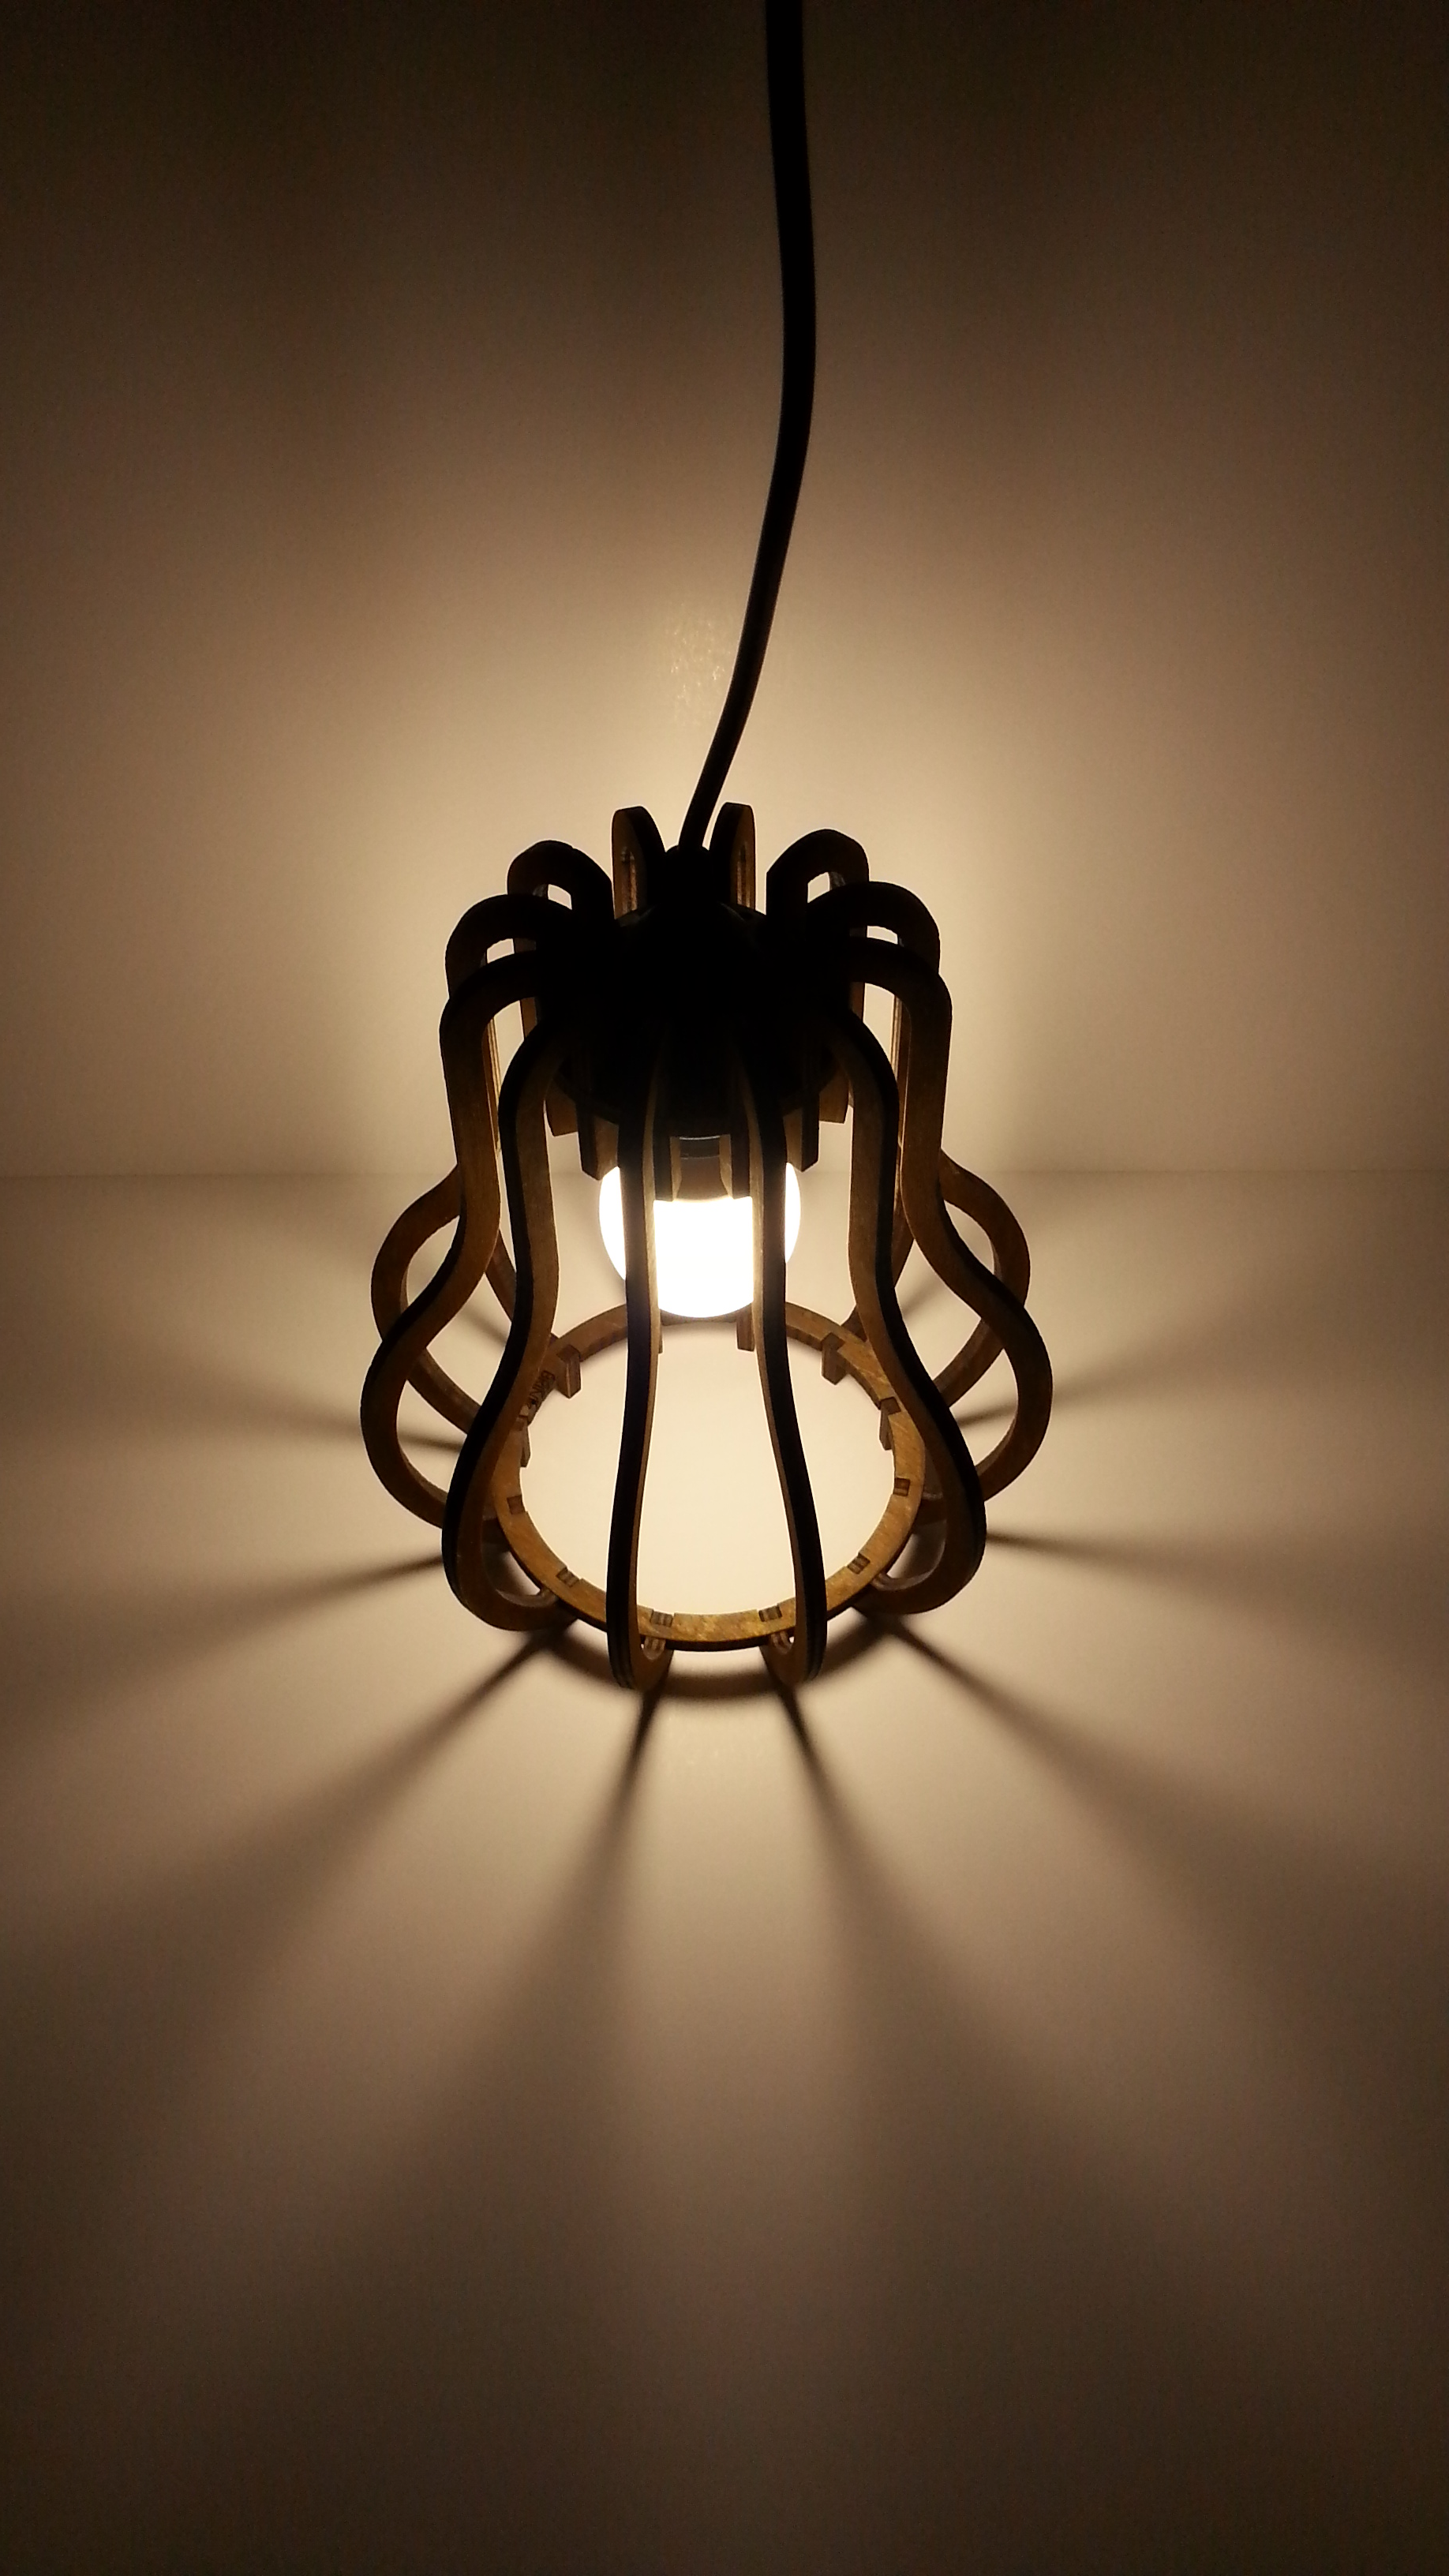
\includegraphics[width=.4\linewidth]{real}
  \caption{}
  \label{fig:real}
\end{subfigure}%
\begin{subfigure}{.5\textwidth}
  \centering
  \includegraphics[width=.4\linewidth]{result_5305s}
  \caption{}
  \label{fig:fake}
\end{subfigure}
\caption{Viser billede taget med mobilkamera (a) og billede renderet af programmet (b). For de to billeder gælder at pærens farvetemperatur er 2700K.}
\label{fig:test_real_fake}
\end{figure}

For at teste de forskellige brugerinput, som kan indtastes i programmet, er der herunder billeder med forskellige brugerinput.

Først testes farvetemperaturen.
\begin{figure}[H]
\centering
\begin{subfigure}{.5\textwidth}
  \centering
  \includegraphics[width=.4\linewidth]{result_5305s}
  \caption{}
  \label{fig:real}
\end{subfigure}%
\begin{subfigure}{.5\textwidth}
  \centering
  \includegraphics[width=.4\linewidth]{result_2734s_5000k_0H_0-785V}
  \caption{}
  \label{fig:fake}
\end{subfigure}
\caption{Viser billede renderet af programmet, med farvetemperaturer på 2700K (a) og 5000K (b).}
\label{fig:farvetemp}
\end{figure}

Herefter sammenlignes billeder renderet med forskellige vinkler.
\begin{figure}[H]
\centering
\begin{subfigure}{.5\textwidth}
  \centering
  \includegraphics[width=.4\linewidth]{result_2734s_5000k_0H_0-785V}
  \caption{}
  \label{fig:real}
\end{subfigure}%
\begin{subfigure}{.5\textwidth}
  \centering
  \includegraphics[width=.4\linewidth]{result_2758s_white_0-8H}
  \caption{}
  \label{fig:fake}
\end{subfigure}
\caption{Viser billede renderet af programmet, med vinkler 0H 0.785V (a) og 0.8H 0V (b).}
\label{fig:synsvinkel1}
\end{figure}

\begin{figure}[H]
\centering
\begin{subfigure}{.5\textwidth}
  \centering
  \includegraphics[width=.4\linewidth]{result53s}
  \caption{}
  \label{fig:real}
\end{subfigure}%
\begin{subfigure}{.5\textwidth}
  \centering
  \includegraphics[width=.4\linewidth]{result658s}
  \caption{}
  \label{fig:fake}
\end{subfigure}
\caption{Viser billede renderet af programmet. Den nye algoritme opnår en speedup på 12 med tiderne 53 Sek[Ny algo] (a) og 658 Sek[Gamel algo med bounding spheres] (b).}
\label{fig:synsvinkel1}
\end{figure}

\subsection*{Opsummering}
Som vist på figur \ref{fig:fake} opfylder programmet krav 1-3 fra afsnit \ref{sec:krav_til_kode}, da den kan rendere og gemme et billede af en lampe og dens belysning på baggrund af indtastede input der indeholder 3D-fil, farvetemperatur, synsvinkel og opløsningen af billedet. Derudover er der som vist sket en optimering af programmets renderingstid efter implementeringen af kd-træer. 
Som det er vist på figur \ref{fig:test_real_fake} er der en afvigelse mellem billedet af den rigtige lampe og det renderede billede af en model af lampen. Denne afvigelse diskuteres i næste afsnit sammen med rapportens resterende resultater. 

%Der er nu blevet udført forskellige test af programmet, som senere diskuteres i afsnit \ref{sec:diskussion}.
\clearpage

\section{Konklusion}
Formålet med dette afsnit er, at opsummere hvordan den endelige problemformulering blev udarbejdet. Derudover konkluderes der hvorvidt den udviklede løsning besvarer den endelige problemformulering.

I problemanalysen, blev der argumenteret for det initierende problems relevans. I denne forbindelse blev der antaget, at det initierende problem eksisterede, på baggrund af egne erfaringer, diskussion med lektor Lars Peter Jensen og en udtagelse fra en belysningskonsulent for en dansk lampebutik. Ønsket var at bekræfte antagelsen ved at udføre en spørgeskemaundersøgelse. Da denne undersøgelse aldrig blev fuldført, er det ikke bevist, at det initierende problem eksisterer.
Efter argumentationen for problemets relevant blev begreber, interessenter og placering af det initierende problem undersøgt. Resultatet af disse undersøgelser dannede grundlaget for den endelige problemformulering.

Det første underspørgsmål i problemformuleringen var: \textit{"Hvordan visualiseres lyset fra en given indendørslampe?"}. Dette underspørgsmål blev besvaret ved at repræsentere lampen, som en 3D-model, som sammen med brugerinput om den ønskede visualisering, indlæses af programmet og renderes vha.\ raytracing med brug af phong-modellen beskrevet i afsnit \ref{sec:teori}.

Det andet underspørgsmål var: \textit{"Hvordan kan lampen og dens belysning visualiseres fra flere vinkler?"}. Dette underspørgsmål blev besvaret ved at anvende teorien om rotationsmatricer i afsnit \ref{sec:teori}, til at positionere det virtuelle kamera, som billedet renderes ud fra.

Det tredje underspørgsmål var: \textit{"Hvordan visualiseres forskellige pærers lys?"}. Her blev der anvendt en algoritme, som konverterer en farvetemperatur for pæren til en RGB-værdi, som kunne benyttes i phong-modellen.

Problemformuleringens overordnede spørgsmål var \textit{Hvordan kan vi lave et værktøj til e-butikker, som visualiserer belysningen fra indendørslamper for kunderne?"}. Ud fra ovenstående kan det nu konkluderes, at problemformuleringen er delvist løst, da der er udviklet et værktøj, der kan visualisere en lampe og dens belysning med forskellige synsvinkler og farvetemperaturer. Problemformuleringen er kun delvist løst, da der stadigvæk er mangler i forhold til implementeringen af værktøjet på en e-butiks hjemmeside. Programmet mangler følgende:

\begin{itemize}
\item Bedre overenstemmelse af farvetemperaturen for pæren i den rigtige lampe i forhold farvetemperaturen på det renderede billede.
\item Lavere renderingstid for, at løsningen er praktisk anvendelig.
\item Brugerflade til visning af billeder.
\end{itemize}

\clearpage

\section{Perspektivering}
I dette afsnit forklares der hvad der skal til for at arbejde videre på løsningen samt alternative anvendelsesmuligheder. 

For at arbejde videre på løsningen kræver det følgende:

\begin{itemize}
\item En brugerflade til visning af billeder på e-butiks hjemmeside.
\item Optimering af raytraceren så renderingstiden formindskes. 
\item Viderudvikling af raytaceren med henblik på højere realisme.
\item Højere overenstemmelse med reel farvetemperatur for pærer.  
\item At lave en backend for kommunikationen mellem serveren hvor billederne renderes og en e-butiks hjemmeside.
\end{itemize}

Selvom løsningsforslaget i denne rapport er målrettet mod kunder som handler lamper på en e-butiks hjemmeside, så er der andre anvendelsesmuligheder for løsningsforslaget. Det kunne tænkes at løsningsforslaget også kunne visualisere lamper og deres belysning for kunder der handler i en detailbutik ved at have en computer eller tablet som har implementeret løsningen. 

I rapporten er det beskrevet, hvordan man kan konstruere et program der renderer et billede på baggrund af en 3D-fil. Denne løsningsmodel kan nødvendigvis ikke kun bruges på lamper, men er også anvendelig til visualisering af andre produkter, som f.eks.\ elektronikprodukter, møbler mm.\ 

\clearpage

\section{Appendiks}
\section*{Projektforslag}
\section*{Produktvisualisering ved e-handel}
I takt med flere og flere computere i individers hjem, er adgangen til internettet blevet større. Grudet dette er e-handelbranchen boomet og har gjort indkøb af forskellige varer meget nemmere, men den er stadig ikke optimal. Et af de største problemer ved e-handel er manglende visualisering af de udbudte produkter. Hvis man leder efter en vare, kan man som regel nemt finde den på en internetside ved en hurtig søgning på internettet, men beskrivelsen er kort, målene er svære at visualisere og man kan ikke forestille sig varen i en given sammenhæng.

\subsection*{Problemstilling}
Hvis køberen ser et produkt, som umiddelbart ser godt ud, og derfor køber det, men grundet manglende visualisering, viser det sig at produktet ikke passer kunden, kan dette skabe en situation, hvor køberen er nødt til at returnere produktet. Dette stiller både sælger, køber og kunde utilfredse. Hvordan kan man hjælpe køberen med at købe et produkt fra en e-handelsbutik, så både kunden og sælgeren opnår den største tilfredshed?

\subsection*{Mål}
Målet er at definere en model, som kan optimere e-handelsbrancen, så f.eks\. fejlkøb undgås, ved hjælp af en eller flere af understående datalogiske problemstillinger.

\subsection*{Ekspempler på datalogiske problemstillinger}
Raytracing, rasterisering, augmented reality.

\subsection*{Ekspempler på kontekstuelle problemstillinger}
Hvilke forskellige metoder er der til visualisering, og hvilke er de mest optimale til at visualisere et givent produkt fra en e-handelsbutik?

\subsection*{Forslagsstiller}
Gruppe B2-28 (SW1b2-28@student.aau.dk)
\clearpage

\bibitem{lamport94}
  Leslie Lamport,
  Addison Wesley, Massachusetts,
  2nd edition,
  1994.
\bibitem{lamport16}
  Leslie Lamport,
  Addison Wesley, Massachusetts,
  2nd edition,
  2016.

\section{Bilag}

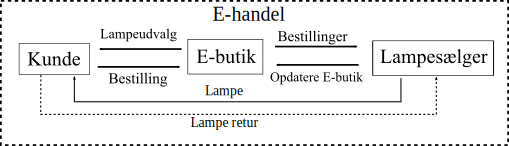
\includegraphics{graphics/e_handel_med_lampe.pdf}

\end{document}
